\documentclass[CMPE]{KGCOEReport}
\usepackage{float}
\usepackage{adjustbox}
\graphicspath{ {./images/} }

\newcommand{\name}{Mohammed Fareed \\ Trent Wesley}
\newcommand{\exerciseNumber}{5}
\newcommand{\exerciseDescription}{MSP432 Timers, Interrupts, and Analog-to-Digital
Converter}
\newcommand{\dateDone}{September 27, 2023}
\newcommand{\dateSubmitted}{October 18, 2023}

\newcommand{\classCode}{CMPE 460}
\newcommand{\LabSectionNum}{1}
\newcommand{\LabInstructor}{Prof.\ Hussin Ketout}
\newcommand{\TAs}{Andrew Tevebaugh \\  Colin Vo}
\newcommand{\LectureSectionNum}{1}
\newcommand{\LectureInstructor}{Prof.\ Hussin Ketout}


\begin{document}
\maketitle

\section*{Abstract}

\section*{Design Methodology}

Interrupts are a useful tool for efficiently handling events by pausing the CPU's current task to handle another. Interrupts provide the benefit of assigning priority to certain events so that they can be executed in a proper order. In addition, interrupts avoid the need to constantly poll, which can interfere with the flow of a program. Interrupts are used extensively in this exercise by timers, switches, UARTs, and GPIO.\\

The MSP432 contains two Timer32 modules for timing operations. Each module contains a counter which can be configured as a 16-bit or 32-bit down counter. In this exercise, C code was written so that pressing Switch1 on the MSP432 microcontroller board activates Timer32-1 which toggles LED1 every 0.5 seconds. To accomplish this, Switch1 was configured to generate interrupts on the falling edge of the button click. The interrupt from a button click starts the interrupt service routine for the switch's port. Within the ISR, the interrupt flag for Switch1 is checked to see if the interrupt came from it. If the interrupt was from Switch1, the state of Timer32-1 gets toggled and a boolean value tracking Timer32-1's state is updated. While Timer32-1 is active, it generates an interrupt every 0.5 seconds. Every interrupt triggers an ISR which checks the state of LED1 with a boolean variable and toggles both the variable and the LED state.\\

More code was written to track time between button presses and cycle an LED through a list of colors. Switch2 on the MSP432 microcontroller board was configured to generate interrupts when pressed. The ISR of Switch2 would first check its interrupt flag to make sure that the interrupt came from it. If Timer32-2 was not already running according to a boolean flag variable, a millisecond counter variable gets set to 0, LED2 gets set to the next color, and a color index variable gets updated. Timer32-2 generates an interrupt every millisecond and triggers an ISR which increments a millisecond counter. If Timer32-2 was running on a Switch2 press, LED2 gets turned off and the UART sends a message of how much time has elapsed based on the millisecond counter. \\

Analog to digital converters are essential for converting real-world data into computer readable digital signals. The MSP432's ADC was used to measure the voltage which varied as the resistance of a photocell changed with light. The circuit in Figure \ref{fig:photocell} was constructed to measure this varying voltage.

\begin{figure}[H]
    \centering
    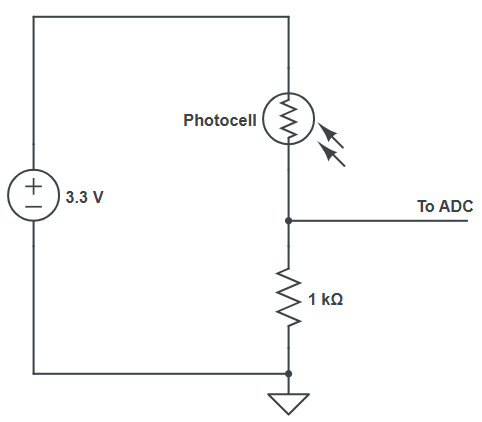
\includegraphics[width=0.4\textwidth]{photocellCircuit.png}
    \caption{Photocell Circuit}
    \label{fig:photocell}
\end{figure}

This circuit shown in Figure \ref{fig:photocell} is a voltage divider circuit with the middle node going to the ADC. The voltage at the middle node follows the behavior shown in Equation \ref{eq:voltageEq}.

\begin{equation}
\text{V}_\text{N} = 3.3V * \frac{1\text{k}\Omega}{1\text{k}\Omega + \text{R}_\text{Photocell}} \label{eq:voltageEq}
\end{equation}

Equation \ref{eq:voltageEq} shows that if the resistance of the photocell increases, the voltage measured by the ADC decreases. Since the resistance of photocell decreases with increased light intensity, it is known that the measured voltage will increase as light intensity increases.

\section*{Results and Analysis}

\section*{Questions}

\section*{Conclusion}

\newpage
\begin{figure}[H]
    \centering
    \begin{adjustbox}{center}
        % 
\includegraphics[width=1.35\textwidth]{signoff.pdf}
    \end{adjustbox}
\end{figure}

\end{document}
